%! Author = borisdeletic
%! Date = 03/05/2023

% Preamble
\documentclass[11pt]{article}


% Document
\begin{document}

    \section{Constrained Hamiltonian Monte Carlo}\label{CHMC}
    Consider the constrained prior distribution subject to the hard likelihood constraint
        \begin{equation}\label{eq:constrained_prior}
            \tilde{\pi}(\theta) =   \begin{cases}
                                          \pi(\theta), & \mathcal{L}(\theta) > \mathcal{L}_0 \\
                                          0, & \text{otherwise}
                                      \end{cases}
        \end{equation}
    Hamiltonian Monte Carlo can be readily adapted to sample from a constrained distribution, making it a viable
    technique for generating new live points in nested sampling.
    As described conceptually by Skilling~\cite{GMC} \& Betancourt~\cite{Betancourt_NS_CHMC}, reflecting
    off the iso-likelihood contours ensures that the proposed sample is within the constrained distribution.
    When the next point in the trajectory would be below the likelihood constraint, we reflect the momentum normal to $\mathbf{n}$ according
    to
    \begin{equation*}
    \begin{aligned}
        \mathbf{p'} &= \mathbf{p} - 2 \frac{ \mathbf{p} \cdot \mathbf{n_R} }{\mathbf{n} \cdot \mathbf{n_R}} \mathbf{n} \\
        \mathbf{n_R} &= M^{-1} \mathbf{n}
    \end{aligned}
    \end{equation*}

    \begin{figure}[t!]
        \center
        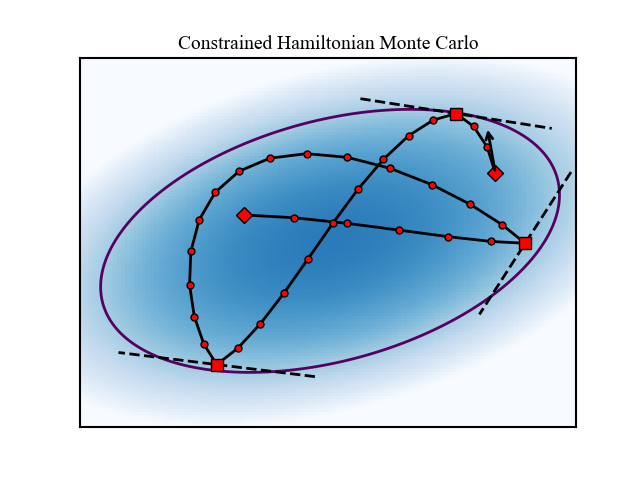
\includegraphics[width=\linewidth]{../figures/ConstrainedHMC}
        \caption{
        Hamiltonian Monte Carlo modified to reflect off iso-likelihood boundaries. Initial point with randomly sampled
        momentum (diamond with arrow) moving in potential well shown in blue. Finite step size $\epsilon$, shows discretisation of
        integrator with intermediate points (circles). Points which reflect off boundary (squares) do not fall exactly on
        the boundary due to discretization. After a fixed number of integration steps $L$, we propose a new sample from the
        constrained distribtion (diamond).
        }\label{fig:constrainedhmc}
    \end{figure}

    Implementing this algorithm in practice poses new challenges with discretization and clustering.
    We propose a novel set of additional algorithms which are essential for a working implementation of
    Constrained HMC (CHMC).

    \subsection{Epsilon Halving}
    When performing reflections with a finite step size $\epsilon$, there is no guarantee that after a reflection,
    the next point will be within the constrained boundary.
    While this scenario is uncommon for smooth boundaries, over many iterations it is likely that at one time,
    no valid reflection will be found, causing the algorithm to crash.

    \begin{figure}[t!]
        \center
        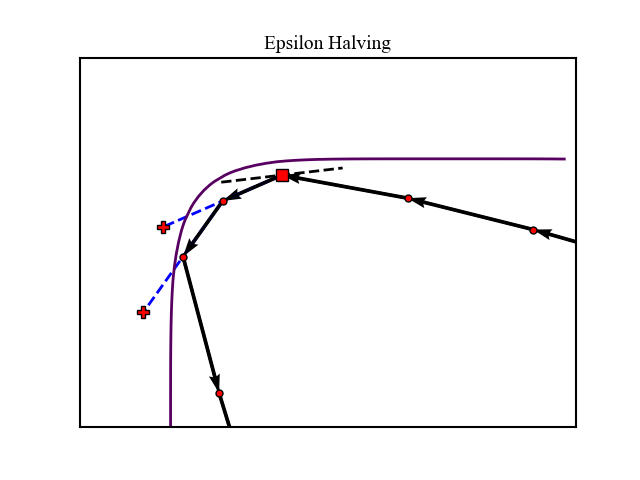
\includegraphics[width=\linewidth]{../figures/EpsilonHalving}
        \caption{
        For sharply curved boundaries, it is possible for the reflected points (plus) to also lie outside the boundary
        constraint, leaving no valid reflections.
        In order for the algorithm to continue, a temporary step size is used to calculate the next position only.
        We iterate $\epsilon' = \epsilon / 2$ until the next point lies within the constraint.
        After a valid point is found, we return back to integrating with $\epsilon_0$.
        }\label{fig:epsilon_halving}
    \end{figure}

    We propose a new reflection scheme which guarantees that a valid reflection will always be found, allowing the
    algorithm to continue.
    After a reflection, the next point is checked to see if it lies outside the boundary.
    If so, a temporary step size $\epsilon' = \epsilon / 2$ is used to re-integrate the position of the next point.
    Epsilon is repeatedly halved until a valid next point is found.
    This is guaranteed to find a valid reflection as the limit $\epsilon' -> 0$ performs a continous reflection.
    The algorithm then continues with the original $\epsilon_0$. \\

    \begin{algorithm}
        \caption{Epsilon Halving}
        \label{alg:epsilon_halving}
        \begin{algorithmic}
            \STATE \COMMENT{Momentum reflection}
            \STATE $\mathbf{p} \gets \mathbf{p} - 2 \left(\mathbf{p} \cdot \hat{ \mathbf{n} } \right) \hat{ \mathbf{n} }$
            \STATE
            \STATE $ \mathbf{x_{new}} \gets \mathbf{x} + \epsilon_0 \mathbf{p}$
            \STATE $ \epsilon' \gets \epsilon_0$
            \WHILE{ $\mathcal{L}(\mathbf{x_{new}}) < \mathcal{L}_0$ }
                \STATE $\epsilon' \gets \epsilon' / 2$
                \STATE $ \mathbf{x_{new}} \gets \mathbf{x} + \epsilon' \mathbf{p}$
            \ENDWHILE
            \STATE $\mathbf{x} \gets \mathbf{x_{new}}$
        \end{algorithmic}
    \end{algorithm}


    \subsection{Ergodicity}
    Ergodicity and detailed balance are well known to be requirements of any MCMC algorithm~\cite{Metropolis_OG}.
    However, in practice no algorithm is truly ergodic due to imperfections in computation such as floating-point
    errors and the cyclic nature of pseudo-random number generators.
    The question then becomes whether the algorithm is \emph{sufficiently ergodic}.
    It is clear the process introduced by epsilon halving is not ergodic, therefore it is essential we ask
    whether our algorithm will maintain sufficient ergodicity.
    Adaptive techniques in MCMC methods have been shown to still converge to the required
    distribution~\cite{MCMC_Ergodicity}.
    Therefore, we argue that so long as our non-ergodic techniques are used infrequently, CHMC will be sufficiently
    ergodic to pass all statistical tests.


\end{document}